%%%%%%%%%%%%%%%%%%%%%%%%%%%
%%%%%%%%%NEWS CRAWLER%%%%%%%%%
%%%%%%%%%%%%%%%%%%%%%%%%%%%
In this chapter we will analyse the two basic components of this work, and we will design a solution in which the output data of the first one (News Crawler \ref{newsCrawler}) will be the input data of the second one (Sentiment Analysis \ref{sentimentAnalysis}). For this we will introduce some simple and general sequential algorithm that will give us a brief overview of how we will deliver our solution.


\begin{algorithm}
\caption{General Algorithm}\label{generalAlgorithm}
\begin{algorithmic}[1]
\FOR {\text{each company}}
	\STATE \text{Crawl News articles;}
	\STATE \text{Extract} \textit{article: date, title, content, author}\text{;}
	\STATE \text{Classify} \textit{article}\text{;}
	\STATE \text{Save} \textit{article}\text{;}
\ENDFOR
\STATE \text{Summarize} \textit{articles}\text{;}
\STATE \text{Download \& Save} \textit{stock prices}\text{;}
\end{algorithmic}
\end{algorithm}

Each part of the algorithm \ref{generalAlgorithm} will take one or several sections in this work, besides is the highest level of abstraction of the tasks that will be performed. This process will be repeated for each of the previously defined companies (see the table \ref{tab:analyzedCompanies}). Basically, we will crawl the news for every company (as shown in section \ref{newsCrawler}) and we will extract the information of our interest (as described in section \ref{locators}), after this we will classify the article in positive or negative (according to the section \ref{sentimentAnalysis}), finally we will be saving every article in our page repository \ref{pageRepository}. When we will finish the iteration, for all companies we will summarise the data and download the stock prices as described in the section \ref{priceRetrieval}. Later, with this data we will perform a statistical analysis (Pearson correlation \ref{PearsonCorr}), based on the assumption that the data that we obtained share a \emph{linear relationship}.


\section{News crawler}\label{newsCrawler}

This section will describe how the task of "news article retrieval" was performed in order to get the right data from the news endpoint.
In a perfect world when every Web application/Web page has its own Web API the "article retrieval" would be a trivial task that would consist on consuming a Web API and we would get structured information, but unfortunately not all web pages allows access to their information through Web API.
We will use as news endpoint "google news"; even if it doesn't have a Web API, because the news articles there, are already categorised by company and date.

By crawling "google news", we will basically get links of articles pointing to different web pages; not articles \emph{per se}. This suppose a problem because every web page has different html structure. So, our crawler must be smart enough to associate one host to one particular page structure. To solve this problem we will introduce the term: Locators, which basically define for every host where is the data that we will extract.

To get this information, we will develop what is called in Liu \cite%[p. 312]
{L2011}: "A focused crawler" \ref{focusedWebCrawling}, where we will focus on \emph{news articles} of a particular company. Besides, we will make several modifications to this algorithm in order to adapt it to our needs. A basic focused web crawler is shown in the figure: \ref{fig:Crawler_002}, our classifier will be based on the fact that we only want news articles, and we will crawl our seed with different parameters (table \ref{tab:query-string}) in order to obtain the desired data.

	\begin{figure}\centering
		\includegraphics[scale=0.3]{Crawler_002}
		\caption{Basic focused web crawler algorithm.}\label{fig:Crawler_002}
	\end{figure}

\begin{algorithm}
\caption{Crawler Algorithm}\label{crawlerAlgorithm}
\begin{algorithmic}[1]
\STATE \text{Set } \textit{timeout;}
\STATE \text{Initialize } \textit{locators;}
\STATE \text{Initialize } \textit{seed(s);}
\STATE \text{Send } \textit{request;}
\STATE \text{Recieve } \textit{response;}
\STATE \text{Parse } \textit{response;}
\STATE \text{Extract } \textit{links} \text{ of our interest;} 
\FOR {\text{each} \textit{link} }
	\STATE \text{Save } \textit{link;}
	\STATE \text{Load } \textit{locator} \text{ for the host;}
	\STATE \text{Extract from} \textit{link: date, title, content, author}\text{;}
	\STATE \text{Save extracted data;}
\ENDFOR
\end{algorithmic}
\end{algorithm}

\subsection{Web Crawler}\label{webCrawler}

According to Liu \cite%[p. 311]
{L2011} a Web crawler is basically a program that automatically download Web pages. To build the Web crawler, we will need a set of seed pages; in our case, our main seed will look like follows: 
\\\\
\url{https://www.google.com/finance/company\_news?q=\%s&start=\%s&num=\%s}
\\\\

	\begin{figure}\centering
		\includegraphics[scale=0.35]{News_001}
		\caption{Screenshot of Google News.}\label{fig:News_001}
	\end{figure}

Every variable in the query string will represent something in particular, as described in  the table \ref{tab:query-string}.

\begin{table}\centering
	\caption{Query string variables}\label{tab:query-string}
   	\begin{tabular}{ | l | p{4cm\textwidth} | p{6cm\textwidth} |}
   	\hline
   	\textbf{Variable}  & \textbf{Explanation} & \textbf{Example}  \\ \hline
    	q & 
	In this variable, we will put the code of a particular company in the stock market.  & 
	Supposing that we want to retrieve all the news of apple(AAPL), the we will send: q=AAPL\\ \hline
	start & 
	This variable define in which index we will start watching the news.  & 
	Assume there are 100 news available, and I want to start in news article number 20; so, we will send: start=20 \\ \hline
	num & 
	This variable define how many news articles I will retrieve in one request. Maximum per request is 50. &
	We could use the previous example, assume we are starting in news article number 20, and we want to see the next 10 articles; so, we will send: start=20 and num=10 \\ \hline
    \end{tabular}
\end{table}

For each company we will generate \textit{N} number of links depending to the number of published articles per company. In every link that we will generate and crawl, we will find news articles links which will be pendant to be visited, these links are called:  \textit{the frontier}; which for efficiency matters and because of its small size (up to 50 links per crawled seed) will be stored in the main memory.

At the end we will have some sort of "preferential crawler"  \cite%[p. 314]
{L2011} due to not all the links of the page will be interesting for us; only the article links. From here, we will extract the article link, date, and title. To get this data we must check deeply the structure of the web page, to figure it out we help ourselves with \emph{Firefox developer tools}, which is a plugin of the Firefox Web browser, it will allow us to know the location (that's why further we will call this part of the application \emph{Locators}) of the element (title, date, link) of our interest. We can see in the figure \ref{fig:News_002} the plugin where we locate the main container of one particular news article. After identifying the container of the news article, we must identify the location of the title of the article, which contain as well the link of the article as shown in the figure \ref{fig:News_003}, and the last part would be to identify the date of the article, as shown in the figure \ref{fig:News_004}. 

	\begin{figure}\centering
		\includegraphics[scale=0.35]{News_002}
		\caption{Container of every article.}\label{fig:News_002}
	\end{figure}
	
	\begin{figure}\centering
		\includegraphics[scale=0.35]{News_003}
		\caption{Title of the article.}\label{fig:News_003}
	\end{figure}
	
	\begin{figure}\centering
		\includegraphics[scale=0.35]{News_004}
		\caption{Date of the article.}\label{fig:News_004}
	\end{figure}

\subsection{Implementation Issues}\label{implementationIssues}
In this section we will describe the "Implementation Issues" that we faced.
%\cite[p. 315]{L2011}
We will use one open-source tool: "jsoup" in order to download and parse a web page, so we will abstract this part, and we will focus on our main aim: news articles.

\subsubsection{Fetching}\label{fetching}
Once we have a particular link, and we will proceed to download the Web page, one important detail must be taken in consideration: \textit{timeout} connections; in the case of the application this parameter will be set to 30 seconds; which of course can be changed in the configuration file that we will call: "jsoup.properties". This part will be delegated to jsoup.

\subsubsection{Parsing}\label{parsing}
Again, the parsing part will be delegated to jsoup. Which manages in a good and efficient way the whole page structure by using "hash tables." In our particular case, once we fetched and parsed the article web page, we need to extract only the data that we are interested in. For this, and as we mentioned at the beginning of this chapter , we will introduce the term: "Locators" in the next section.

\subsubsection{Locators}\label{locators}
The aim of the "news crawler" is basically to extract \textit{title, date, author, content} from a particular article, and if we take in consideration that every Web page has \emph{different structure}, we need to define an extra component in order to extract accurately the information that we needed. We must mention that this method is very accurate when it tries to retrieve the article data.

We will define a Locator as a custom data structure that holds the particular representation of the structure of a web page in a particular host, in order to retrieve the data that we want. For this purpose a class can be found under the package: "com.carramil.dp.crawler" called: "Locator.java", and this class has its input data in a properties file which we called: "crawler.properties". The structure of this file is as follows: We will enumerate \textit{N} number of hosts from 1 to \textit{N} and for each of them we will define the required information as shown in the table: \ref{tab:locator}. Each item between semi-colons is a path to a particular tag; if we want to specify a path we must do it by separating every tag with "-$>$". It is important to mention that there must not be blank spaces between each semi-colon (";"), and in the case one particular host has several different page structures we can use ampersand ("\&") to separate between tags. We will mention an example in order for this part to be clear.

\begin{table}\centering
	\caption{Locator format}\label{tab:locator}
   	\begin{tabular}{p{11.5cm}}
   	\hline
GenericCrawler.source.1 = host;title;content;author;date;dateFormat\\
GenericCrawler.source.2 =host;title;content;author;date;dateFormat\\
GenericCrawler.source.3 =host;title;content;author;date;dateFormat\\
... up to \textit{N} ...\\
GenericCrawler.source.\textit{N} =host;title;content;author;date;dateFormat\\
    \hline
    \end{tabular}
\end{table}

\begin{table}\centering
	\caption{Locator example}\label{tab:locatorExample1}
   	\begin{tabular}{p{11.5cm}}
\lstset{language=HTML}
\begin{lstlisting}
<!DOCTYPE html>
<html>
<head>
    <title>my Page title</title>
</head>
<body>
	<div id="menu">
		The menu of the Web Page
	</div>
	<div class="meta-data">
		<h1>Title of the article</h1>
		<div class="author">
			By: <a href="#">Author Name of this article</a>
		</div>
		<div class="dateTime myFormat">
			Oct 9, 1985
		</div>
	<div >
	<div id="articleBody">
		This will be the body of the article
	</div>
</div> 
</body>
</html>
\end{lstlisting}
    \end{tabular}
\end{table}

In this example listed in the table: \ref{tab:locatorExample1} we will identify each of the things that we will be interested in, we will start with title: "body-$>$div.meta-data-$>$h1" and the result according to the example would be "Title of the article", we could define the locator by just specifying the tag "h1", because in this case the tag is unique in the document.

To get the content of the article we can construct the following locator: "body-$>$div\#articleBody" or as mentioned before "div\#articleBody" works for our purposes.

To get the date of the article the locator follows the pattern: "body-$>$div.meta-data-$>$div.dateTime.myFormat", and we have to specify to the Locator the format of this date; in this case is: MMM dd, yyyy. Remember that we can specify more than one date format.

The author would be retrieved as follows: "body-$>$div.meta-data-$>$div.author-$>$a".

Once we have this information from a particular host, the complete locator would be:\\
\emph{
GenericCrawler.source.1 = "www.host.com;body-$>$div.meta-data-$>$h1;\\
body-$>$div\#articleBody;body-$>$div.meta-data-$>$div.author-$>$a;\\
body-$>$div.meta-data-$>$div.dateTime.myFormat;MMM dd, yyyy"
}
\\\\
An actual example of a Locator:

\emph{
"GenericCrawler.source.2 = www.reuters.com;h1;\\
span\#articleText\&div.columnLeft-$>$p;p.byline;span.timestamp;\\
EEE MMM dd, yyyy hh:mma z\&dd MMM yyyy\&\\
MMM dd, yyyy\&EEE, dd MMM yyyy\&EEEE, MMM dd yyyy"}

But how to create a locator? we make a reference to \ref{crawlerProperties} in order to make an example on how to create one locator. And we will recall the \emph{Locator} of one particular how: \url{http://www.fool.com}, and we will use the following article to state the example:\\\ \url{Fool.com/investing/general/2014/04/29/apple-incs-ipad-identity-crisis.aspx}

\begin{itemize}
	\item First of all, we will consider the previously mentioned url, it looks like in figure \ref{fig:Locator_001}.
	
\begin{figure}\centering
	\includegraphics[scale=0.4]{Locator_001}
	\caption{Initial Web page.}\label{fig:Locator_001}
\end{figure}
	
	\item Then we must identify where is the location of the header/title of the news article. In our case, because \emph{h1} is an unique location in the webpage, we can just add \emph{h1} or we can add the complete path to it: \emph{body-$>$h1.xlHeader}, as shown in figure \ref{fig:Locator_002}.
	
\begin{figure}\centering
	\includegraphics[scale=0.4]{Locator_002}
	\caption{Retrieving the title.}\label{fig:Locator_002}
\end{figure}
	
	\item After this, we would like to know the location of the content of the news article. Here, again \emph{div.entry-content} is a unique location the webpage, or if we want to be more specific, we would write: \emph{body-$>$div.entry-content} as shown in figure \ref{fig:Locator_003}.

\begin{figure}\centering
	\includegraphics[scale=0.4]{Locator_003}
	\caption{Retrieving the content.}\label{fig:Locator_003}
\end{figure}

	\item Another important thing is the date of the article; as show in the figure \ref{fig:Locator_004}, in order to identify the location of the tag, we must define it as follow: \emph{body-$>$p.articleMeta-$>$span.datetime}.
	
\begin{figure}\centering
	\includegraphics[scale=0.4]{Locator_004}
	\caption{Retrieving the date.}\label{fig:Locator_004}
\end{figure}
	
	\item And last but not least, the author; we must identify the location in the content of the document. Which according to the figure \ref{fig:Locator_005} is: \emph{body-$>$span[itemprop=author]}.
	
\begin{figure}\centering
	\includegraphics[scale=0.4]{Locator_005}
	\caption{Retrieving the author.}\label{fig:Locator_005}
\end{figure}
	
\end{itemize}

\subsubsection{Generic Locator}\label{genericLocator}

When we think about the scalability of the locators (\ref{locators}), is quite poor; not because it does not fulfil its purpose, but because for every site, we \emph{must} examine the structure of the web page, and this \emph{manual} task takes around 5-10 minutes per site. And, while more news sources we would like to have, more time we should spend constructing our locators. 

So, we have to come out with another method, that allow us to retrieve news article from different sources without spending time examining the structure of every news provider. For us, this method will be called \emph{Generic Locators}. 

To implement this method we will refer first to the section \ref{webCrawler}, and we will take advantage that we already know the date, and title of the article. So we will perform a simple heuristic that will let us retrieve significantly more articles; around 40 \% (According experimental results) if we compare it with the total number of articles retrieved.

As usual, when heuristics are applied, we have to do some trade-off in order to get a good solution with an specific algorithm. In our case, our trade-off will be the accuracy of the text of the article; because sometimes we will get some undesirable characters/phrases in the content of the article. Everything will depend on homogeneous and uniform the structure of the webpage is.

\begin{figure}\centering
	\includegraphics[scale=0.4]{GenericLocator_1}
	\caption{Web page without Locator defined}\label{fig:GL_1}
\end{figure}

We will state an example in order to make it clear. Let's consider this link \url{http://gulfbusiness.com/2014/04/apple-seeks-decisive-us-court-ruling-samsung/} (Figure: \ref{fig:GL_1}). So far, we have implemented a Locator in order to crawl this host and gain 100\% of accuracy. So, in this case that's when the \emph{Generic Locator} comes to play. The text that a \emph{Locator} would retrieve would be the following: 
\\\\
\emph{"Apple and Samsung return to \textbf{federal court} on Tuesday for opening statements in their latest patent battle, with the iPhone maker expected to present \textbf{more detailed} evidence in its attempt to win a U.S. ban on sales of several Samsung smartphones.Apple Inc and Samsung Electronics Co (...)
% Ltd have been litigating around the world for nearly three years. Jurors awarded the iPhone maker about \$930 million after a 2012 trial in San Jose, California, but Apple failed to persuade U.S. District Judge Lucy Koh to issue a \textbf{permanent injunction} against the sale of Samsung phones.A sales ban would be a far \textbf{more serious} threat to Samsung, which earned \$7.7 billion in the quarter that ended in December. Samsung’s \textbf{mobile division}, which includes smartphones, generated operating profit of 5.47 trillion won (\$5.1 billion).The two companies are set to embark on another trial in San Jose over a \textbf{fresh batch} of Apple patents, which cover iPhone features like slide to unlock and search technology. Apple is seeking to ban sales of several Samsung phones, including the Galaxy S III.Likewise, Samsung claims Apple violated two of its patents, and is seeking to ban the iPhone 5. Samsung’s phones use the Android operating system developed by Google Inc.In rejecting Apple’s \textbf{previous bid} for a sales ban, Koh wrote that a consumer survey Apple submitted in the 2012 trial \textbf{likely inflated} the value that customers place on the smartphone features in dispute, meaning Apple does \textbf{not merit} an injunction. Apple is appealing that decision.Apple has hired the \textbf{same marketing} expert to conduct a \textbf{new consumer} survey for the \textbf{current trial}. But this latest effort contains \textbf{additional analysis} about how Apple’s patented features drive consumer demand, according to court filings.While the \textbf{prior survey} \textbf{only concluded} that there was \textbf{general demand} for the patented features, the \textbf{new study} attempts to quantify the proportion of customers Samsung would have lost if its smartphones did \textbf{not contain} those features, court filings show.Samsung tried to stop Apple from presenting that evidence to the jury, arguing that the methodology was unsound. 
However, Koh agreed in a February ruling to allow Apple to use the study.The trial is expected to last until early May.The case in U.S. District Court, Northern District of California is Apple Inc vs Samsung Electronics Co Ltd, 12-630."}
\\\\
And in the case of the generic locator we got: 
\\\\
\emph{\ul{Home \/ Technology \/ World Apple Seeks Decisive US Court Ruling Against Samsung Apple and Samsung have been litigating around the world for nearly three years. By Reuters April 1, 2014} Apple and Samsung return to \textbf{federal court} on Tuesday for opening statements in their latest patent battle, with the iPhone maker expected to present \textbf{more detailed} evidence in its attempt to win a U.S. ban on sales of several Samsung smartphones.Apple Inc and Samsung Electronics Co  (...)
% Ltd have been litigating around the world for nearly three years. Jurors awarded the iPhone maker about \$930 million after a 2012 trial in San Jose, California, but Apple failed to persuade U.S. District Judge Lucy Koh to issue a \textbf{permanent injunction} against the sale of Samsung phones.A sales ban would be a far \textbf{more serious} threat to Samsung, which earned \$7.7 billion in the quarter that ended in December. Samsung’s \textbf{mobile division}, which includes smartphones, generated operating profit of 5.47 trillion won (\$5.1 billion).The two companies are set to embark on another trial in San Jose over a \textbf{fresh batch} of Apple patents, which cover iPhone features like slide to unlock and search technology. Apple is seeking to ban sales of several Samsung phones, including the Galaxy S III.Likewise, Samsung claims Apple violated two of its patents, and is seeking to ban the iPhone 5. Samsung’s phones use the Android operating system developed by Google Inc.In rejecting Apple’s \textbf{previous bid} for a sales ban, Koh wrote that a consumer survey Apple submitted in the 2012 trial \textbf{likely inflated} the value that customers place on the smartphone features in dispute, meaning Apple does \textbf{not merit} an injunction. Apple is appealing that decision.Apple has hired the \textbf{same marketing} expert to conduct a \textbf{new consumer} survey for the \textbf{current trial}. But this latest effort contains \textbf{additional analysis} about how Apple’s patented features drive consumer demand, according to court filings.While the \textbf{prior survey} \textbf{only concluded} that there was \textbf{general demand} for the patented features, the \textbf{new study} attempts to quantify the proportion of customers Samsung would have lost if its smartphones did \textbf{not contain} those features, court filings show.Samsung tried to stop Apple from presenting that evidence to the jury, arguing that the methodology was unsound. 
However, Koh agreed in a February ruling to allow Apple to use the study.The trial is expected to last until early May.The case in U.S. District Court, Northern District of California is Apple Inc vs Samsung Electronics Co Ltd, 12-630. \ul{Get your Free Gulf Business Newsletter}}
\\\\
In the last article we can observe the underlined text, which corresponds to the extra-text retrieved by the \emph{heuristic method (Generic Locator)}. And the text in the bold letters represents the part of speech extracted from the text, in this case doesn't affect the \emph{polarity} of the document. For the first document we had a negative score: -1.06451389862862 and for the second one 0.33956281372088865, according to the equations \ref{eq:ourRange1} and \ref{eq:ourRange2} that defines the criteria to assign the polarity to a document. In this case, both documents have \emph{negative polarity}; but why the different scores for each document if both of them states "almost" the same? The answer to this question is quite simple in this case, the word that makes the biggest impact of the score is on the underlined part of the second document: \ul{Get your \emph{Free} Gulf Business Newsletter}. If we check our file of \emph{positve bag of words}  \cite{M1995} in the line 797, there is the word \emph{Free} which is considered as part of the analysis and it will contribute to the average result in a positive way.
\\\\
We will now describe the \emph{Generic locator algorithm} (\ref{genericLocatorAlgorithm}), which basically takes the \emph{title, date, link and host} and verify if there is an actual locator that can process the web page accurately, then we must check if the link is already in our \emph{page repository}, after this, we will download the article and find the \emph{tag} that contains the \emph{title}, if we found it we will assign the \emph{tag} as \emph{parent} and we will iterate until we fulfill the condition of the \emph{minimum article lenght} (determined experimentally; around 200 characters) and on every iteration we will prepare for the next one, we will assign to the variable \emph{article\_text} the text of the current parent and to \emph{article\_length} the length of the parent, and we will update the \emph{parent} to its \emph{parent}.

\begin{algorithm}
\caption{Generic locator algorithm}\label{genericLocatorAlgorithm}
\begin{algorithmic}[1]

\STATE Input: companyId, title, date, link, host;
\STATE Output: article\_text;
\STATE $article\_lenght \gets 0$;
\STATE $article\_text \gets NULL$;
\STATE $min\_article\_lenght \gets 0$;
\STATE $parent \gets NULL$;
\STATE $tag \gets NULL$;

\IF{\neg $host\_has\_locator}
	\IF{\neg $is\_link\_saved}
		\STATE download \emph{article};
		\STATE find \emph{tag} that contains \emph{title};
		\IF{is\_tag\_found}
			\STATE $parent \gets tag$;
			\WHILE{$article\_lenght < min\_article\_lenght$} 
				\STATE $article\_text \gets parent.text()$
				\STATE $article\_lenght \gets length(article\_text)$
				\STATE $parent \gets parent.parent()$
			\ENDWHILE		
		\ELSE
			\RETURN \emph{NULL};
		\ENDIF
	\ENDIF
\ENDIF
\RETURN $article\_text;

\end{algorithmic}
\end{algorithm}

\subsubsection{Page repository}\label{pageRepository}
Once that the page is fetch and parsed, according to Liu \cite%[p. 321]
{L2011}, it may be stored/indexed. In our case, we will need such a particular repository. Mostly because we are not interested in the web page \emph{per se}, but in its content; as we mention in the subsection \ref{locators}. We could have chosen any particular storage method; file system, document oriented database, object oriented database, but for the purposes of this work we will use a relational database: MySQL because for the following reasons:

\begin{itemize}
    \item The information that we are interested in, is just text.
    \item Several transactions will be executed simultaneously.
    \item Complex queries will be performed.
    \item Stored procedures capabilities.
    \item Summarisation operations will be performed quite often.
\end{itemize}

The database server has the following characteristics:

\begin{itemize}
    \item Server: Localhost via UNIX socket
    \item Software: MySQL
    \item Software version: 5.5.29 - Source distribution
    \item Protocol version: 10
    \item Server charset: UTF-8 Unicode (UTF8)
\end{itemize}

For all the news articles that will be saved in the database, it is important to clarify that no HTML will be stored, mostly because it is not the aim of the work. We will be saving the following fields: Title of the article, content of the article, link, post date, author (not mandatory) and web site. Basically we will index the database by link and by post date of the article. If in the future the original article needs to be checked, the link will be stored.

\subsubsection{Concurrency}\label{concurrency}

Once again, we will make a reference to Liu, \cite%[p. 322]
{L2011}. A crawler basically consumes three main resources: network, CPU and disk. 

In the previous sections we have described basically a sequential crawler, and of course, even if we are really good programmers, and we manage to develop and implement an optimum algorithm, as we mention in the last paragraph, there will be some parameters that will make a bottleneck of our sequential application. 



To state an example we will assume the following: 
\begin{itemize}
    \item A web page that weights around 800 KB
    \item a connection of 256 Kbps
\end{itemize}

According to the figure \ref{fig:Bandwidth} in which we have represented the average download time without considering the \emph{overhead}, it will take around 25 seconds. We could think that this download time is not that bad if we try to download only several web pages; but if we think about it deeply, when we try to download maybe hundreds, thousands or maybe millions, this 25 seconds become a huge overhead. And even for the one page case, this 25 seconds for the processor/CPU seems like ages of waiting, and it will depend on the number of cycles per seconds that the CPU can process, in the example in the table: \ref{tab:downloadIdleness} we have consider a single CPU of 2 GHz (2,000,000,000 cycles every second), and as we can see the idleness of the processor (assuming that the processor is not doing anything else but processing our download request) is quite big and it decreases while we have a faster download speed, but even with today's highest commercial bandwidths available, the idleness of the CPU would be quite high.

\begin{table}\centering
	\caption{Download time \& CPU Idleness}\label{tab:downloadIdleness}
   	\begin{tabular}{ | p{2.5cm\textwidth} | p{3cm\textwidth} | p{3.5cm\textwidth} |}
   	\hline
   	\textbf{Bandwidth (Kbps)}  & \textbf{Download time (seconds)} & \textbf{CPU Idleness (Cycles/second)}  \\ \hline

	9.66&666&1,332,000,000,000\\ \hline
	14.4&441&882,000,000,000\\ \hline
	28.8&222&444,000,000,000\\ \hline
	33.6&190&380,000,000,000\\ \hline
	56&114&228,000,000,000\\ \hline
	64&100&200,000,000,000\\ \hline
	128&50&100,000,000,000\\ \hline
	256&25&50,000,000,000\\ \hline
	512&12&24,000,000,000\\ \hline
	1024&6&12,000,000,000\\ \hline

    \end{tabular}
\end{table}

According to Liu \cite%[p. 322]
{L2011}: the most straightforward way to \emph{speed-up} a crawler is through concurrent processes or threads. Multiprocessing may be somewhat easier to implement than multithreading depending on the programming language and platform.

\begin{figure}\centering
	\caption{Web page download}\label{fig:Bandwidth}
	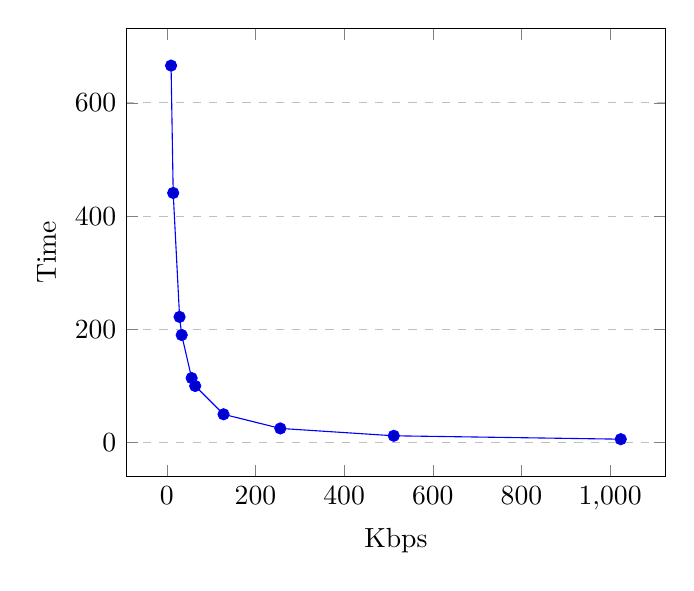
\begin{tikzpicture}
		\begin{axis}[ 
			xlabel=Kbps,
			ylabel=Time,
			ymajorgrids=true,
			grid style=dashed,
  				]	 
			\addplot coordinates {
				(9.6, 666 )
				(14.4, 441)
				( 28.8, 222 )
				(33.6, 190 )
				(56, 114)
				(64, 100)
				(128, 50)
				(256, 25)
				(512, 12)
				(1024, 6)
				};
		\end{axis}
	\end{tikzpicture}
\end{figure}


\begin{figure}\centering
	\caption{CPU Idleness}\label{fig:CPUIdleness}
	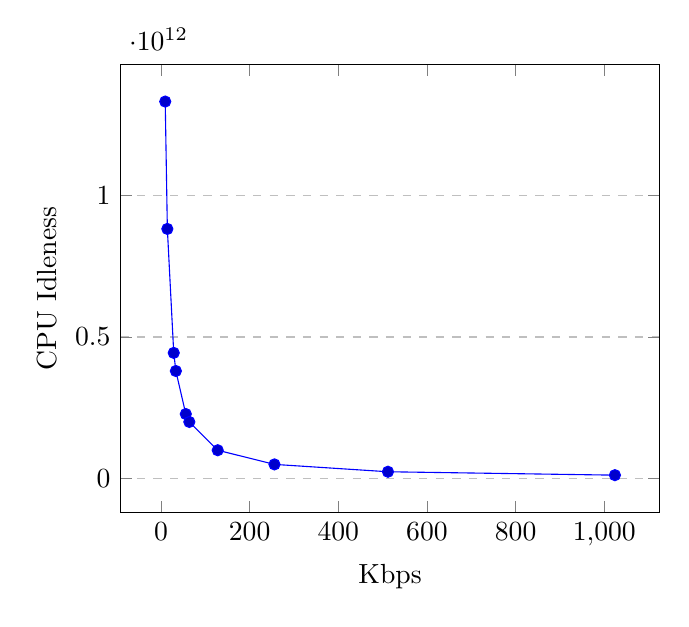
\begin{tikzpicture}
		\begin{axis}[ 
			xlabel=Kbps,
			ylabel=CPU Idleness,
			ymajorgrids=true,
			grid style=dashed,
  				]	 
			\addplot coordinates {
				(9.6, 1332000000000 )
				(14.4, 882000000000)
				( 28.8, 444000000000 )
				(33.6, 380000000000 )
				(56, 228000000000)
				(64, 200000000000)
				(128, 100000000000)
				(256, 50000000000)
				(512, 24000000000)
				(1024, 12000000000)
				};
		\end{axis}
	\end{tikzpicture}
\end{figure}

This word for us (\emph{speed-up}) will have a deeper meaning in the chapter \ref{experimentalEvaluation}, where we will show experimentally the decrease of the idleness of the CPU and the threshold of the parallelisation of the crawler.

In our particular case, we have to make reference to the sequential solution which basically iterates every company until it reaches the last one, after this the collected information is summarised. This approach has the worst time execution (remember: \ref{ParTime}), but of course the best efficiency (remember: \ref{ParEfficiency}); this is represented in the figure \ref{fig:Sequential_1}.

When we will talk about the parallel solution, we will create a pool of requests where we will push the tasks for every company and the framework itself will identify the number of processors available, and it will start to process a set of requests according to the hardware resources available; then it will wait until the last company is processed; this is related to the concept of \emph{Barrier synchronization} (\ref{BarrierSynchronization}). In this case, there will be a threshold where the time will be the best and the speedup as well will be the best; this will be demonstrated experimentally in the chapter \ref{experimentalEvaluation} in the section \ref{MultiThreadingPerformance} specifically in the table \ref{tab:threadsTime}. The idea of the parallel algorithm is depicted in the figure: \ref{fig:Concurrency_1}, and the pseudocode is described in the algorithm \ref{parallelCrawlerAlgorithm} which is implemented in the file \emph{CrawlerThreadPool.java}, this will be the starting point of the console application.

\begin{algorithm}
\caption{Parallel Crawler Algorithm}\label{parallelCrawlerAlgorithm}
\begin{algorithmic}[1]
\STATE \text{Initialize the thread pool;}
\STATE \text{Insert the companies in the thread pool;}
\FORALLP {\text{companies}}
	\STATE \text{Apply the general sequential algorithm \ref{generalAlgorithm};}
\ENDFOR
\STATE \text{Wait until the last task is done (Barrier \ref{BarrierSynchronization}) ;}
\STATE \text{Summarize} \textit{articles}\text{;}
\STATE \text{Download \& Save} \textit{stock prices}\text{;}
\end{algorithmic}
\end{algorithm}


\begin{figure}\centering
	\includegraphics[scale=0.4]{Sequential}
	\caption{Sequential diagram}\label{fig:Sequential_1}
\end{figure}

\begin{figure}\centering
	\includegraphics[scale=0.4]{Concurrency}
	\caption{Model of the parallel solution.}\label{fig:Concurrency_1}
\end{figure}


